% ==============================================================================
% compare_equipo_01.tex
% Presentación "Algorithm Comparison": cómo se compara el mejor modelo con las
% demás familias de algoritmos. Las diapositivas c01 a c10 de comunes/ también
% están en best_equipo_01.tex.
% Compilar desde esta carpeta: pdflatex compare_equipo_01.tex (dos veces).
% ==============================================================================
\documentclass[aspectratio=169, 11pt]{beamer}
% ==============================================================================
% preambulo.tex
% Preámbulo común de las dos presentaciones (best_equipo_01 y compare_equipo_01).
% Las figuras y tablas se toman de 03_Output, donde las generan los scripts del
% repositorio, y las cifras citadas vienen de 03_Output/Tables/pres_cifras.tex
% (01_Scripts/04_Results/03_figuras_presentaciones.R).
% ==============================================================================
\usepackage[T1]{fontenc}
\usepackage[utf8]{inputenc}
\usepackage{lmodern}
\usepackage{graphicx}
\usepackage{booktabs}
\usepackage{tikz}
\usetikzlibrary{positioning, arrows.meta}

\graphicspath{{../03_Output/Figures/}}
\newcommand{\maeprivado}{151,5}
\newcommand{\preciotipico}{806}
\newcommand{\maepctprecio}{19\%}
\newcommand{\ntrain}{36.407}
\newcommand{\nrawtrain}{38.644}
\newcommand{\ncopias}{2.237}
\newcommand{\ntest}{10.286}
\newcommand{\nchaptrain}{305}
\newcommand{\pcttestchap}{94\%}
\newcommand{\preciomdchap}{750}
\newcommand{\preciomdresto}{550}
\newcommand{\aptotest}{97\%}
\newcommand{\aptotrain}{75\%}
\newcommand{\sinareatest}{44\%}
\newcommand{\sinareachap}{6\%}
\newcommand{\coordredondeada}{52\%}
\newcommand{\coordredtrain}{40\%}
\newcommand{\nvarexternas}{61}
\newcommand{\nvartexto}{44}
\newcommand{\ntopicos}{15}
\newcommand{\nenvios}{25}
\newcommand{\margenchap}{19\%}
\newcommand{\sobreestimachap}{46\%}
\newcommand{\sobrediezchap}{25\%}
\newcommand{\pctverde}{11\%}
\newcommand{\pctamarillo}{61\%}
\newcommand{\pctrojo}{27\%}
\newcommand{\mejormargen}{17\%}
\newcommand{\gananciacien}{1.153}
\newcommand{\negociosmargen}{42\%}
\newcommand{\descuentomax}{15\%}
\newcommand{\pasoentorno}{96}
\newcommand{\pasoxgb}{37}
\newcommand{\pasotexto}{13}
\newcommand{\ventajaxgb}{39}
\newcommand{\ventajaensamble}{3}
\newcommand{\mismabasedif}{58}
\newcommand{\cartdistintos}{59}
\newcommand{\sesgobarato}{17\%}
\newcommand{\sesgocaro}{19\%}


% Colores
\definecolor{azul}{HTML}{2166AC}
\definecolor{rojo}{HTML}{B2182B}
\definecolor{verde}{HTML}{1A9850}
\definecolor{gris}{HTML}{595959}
\definecolor{grisclaro}{HTML}{F2F2F2}

% Tema sobrio: títulos en azul, sin íconos de navegación, número de página
\usetheme{default}
\setbeamertemplate{navigation symbols}{}
\setbeamercolor{frametitle}{fg=azul}
\setbeamerfont{frametitle}{series=\bfseries, size=\large}
\setbeamercolor{title}{fg=azul}
\setbeamerfont{title}{series=\bfseries}
\setbeamercolor{structure}{fg=azul}
\setbeamertemplate{itemize items}[circle]
\setbeamertemplate{footline}{%
  \hfill\textcolor{gris}{\scriptsize Equipo 1 \quad \insertframenumber/\inserttotalframenumber}\hspace{1em}\vspace{0.6em}}

% Cifra grande con su descripción. El argumento opcional es el ancho (por
% defecto, un tercio del ancho de la diapositiva).
\newcommand{\cifra}[3][0.3\textwidth]{%
  \begin{minipage}[t]{#1}\centering
    {\Huge\bfseries\color{azul}#2}\\[0.3em]
    {\small\color{gris}#3}
  \end{minipage}}

% Cifra mediana, para acompañar un mapa sin quitarle espacio
\newcommand{\cifrachica}[2]{%
  {\LARGE\bfseries\color{azul}#1}\\[0.1em]
  {\footnotesize\color{gris}#2}}

% Mensaje corto debajo de una figura
\newcommand{\lectura}[1]{\par\vspace{0.2em}{\scriptsize\color{gris}#1}}

% Diapositivas de mapa vertical: el mapa ocupa toda la altura a la izquierda y
% el título va arriba de la columna derecha, con el mismo estilo de los demás
% títulos. \altomapa es la altura del mapa.
\newcommand{\altomapa}{1.02\textheight}
\newcommand{\titulolateral}[1]{%
  {\usebeamerfont{frametitle}\usebeamercolor[fg]{frametitle}#1\par}\vspace{0.9em}}
\newcommand{\mapavertical}[1]{\vspace*{-0.4em}\includegraphics[height=\altomapa]{#1}}

% Figura ancha que usa casi todo el ancho de la diapositiva
\newcommand{\figuraancha}[2][0.97]{\makebox[\textwidth]{\includegraphics[width=#1\paperwidth]{#2}}}


\title{¿Por qué gana el boosting, y por qué importa cómo se valida?}
\subtitle{Precios de vivienda en Chapinero: comparación de algoritmos}
\author{Equipo 1: Mauricio Aragón, Jonathan Cadena y Esteban Flórez}
\date{Big Data y Machine Learning para Economía Aplicada (MECA 4107)\\Universidad de los Andes, 2026-20}

\begin{document}

\begin{frame}[plain]
  \titlepage
\end{frame}

% --- El mejor modelo y el problema --------------------------------------------
% C1. Resultado del mejor modelo (inicio obligatorio de las dos presentaciones)
\begin{frame}{El mejor modelo se equivoca en \maeprivado{} millones por vivienda}
  \centering
  \cifra{\maeprivado{} M}{MAE privado en Kaggle\\(envío 29, ensamble de XGBoost)}\hfill
  \cifra{\maepctprecio}{del precio típico predicho\\en Chapinero (\preciotipico{} M)}\hfill
  \cifra{\nenvios}{envíos a Kaggle con\\seis familias de algoritmos}

  \vspace{1.6em}
  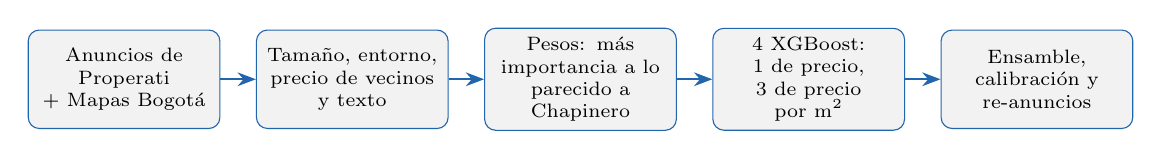
\begin{tikzpicture}[node distance=0.45cm,
      caja/.style={draw=azul, fill=grisclaro, rounded corners, align=center,
                   font=\scriptsize, minimum height=1.25cm, text width=2.2cm},
      flecha/.style={-{Stealth}, thick, azul}]
    \node[caja] (datos) {Anuncios de\\Properati\\+ Mapas Bogotá};
    \node[caja, right=of datos] (vars) {Tamaño, entorno,\\precio de vecinos\\y texto};
    \node[caja, right=of vars] (pesos) {Pesos: más\\importancia a lo\\parecido a Chapinero};
    \node[caja, right=of pesos] (xgb) {4 XGBoost:\\1 de precio,\\3 de precio\\por m$^2$};
    \node[caja, right=of xgb] (ens) {Ensamble,\\calibración y\\re-anuncios};
    \draw[flecha] (datos) -- (vars);
    \draw[flecha] (vars) -- (pesos);
    \draw[flecha] (pesos) -- (xgb);
    \draw[flecha] (xgb) -- (ens);
  \end{tikzpicture}
  \note{El MAE es el error absoluto medio: en promedio el precio predicho se aleja \maeprivado{} millones del precio de venta, cerca de \maepctprecio{} del precio típico. El modelo combina cuatro XGBoost: uno predice el precio y tres el precio por metro cuadrado. El envío también probó agregar modelos con embeddings del texto, pero el ensamble les dio un peso de casi cero, así que en la práctica es un ensamble de XGBoost. Los pesos hacen que el modelo aprenda más de los anuncios parecidos a los de Chapinero. Los re-anuncios son viviendas de test que ya aparecían en train con otra publicación.}
\end{frame}

% C2. El reto: train en toda Bogotá, test en Chapinero
\begin{frame}{El reto: predecir donde casi no hay datos}
  \begin{columns}[c]
    \begin{column}{0.5\textwidth}\centering
      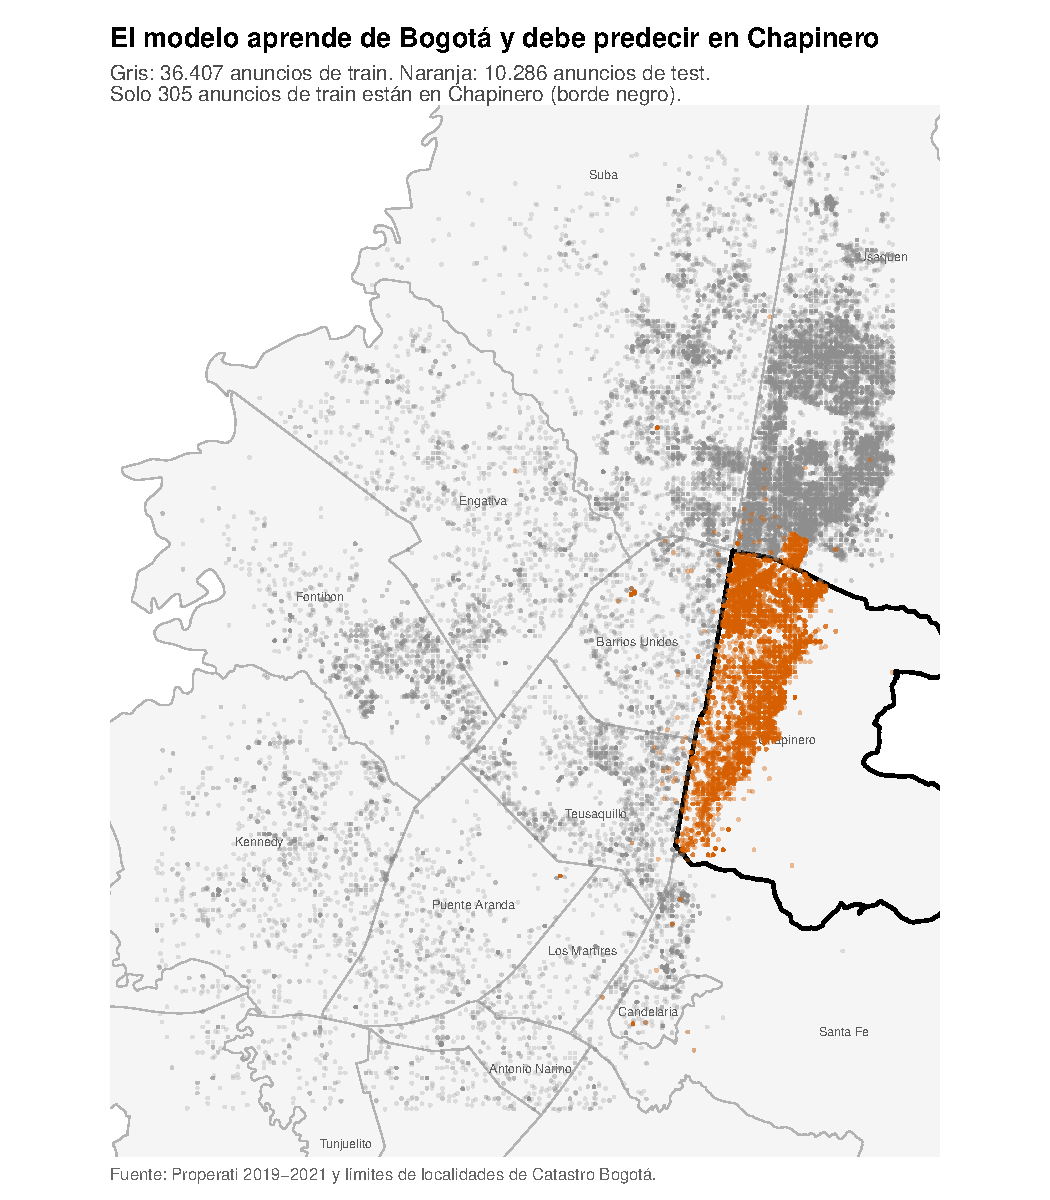
\includegraphics[height=0.82\textheight]{mapa_01_train_test.pdf}
    \end{column}
    \begin{column}{0.45\textwidth}
      \cifra[\linewidth]{\ntrain}{anuncios de train en toda Bogotá}\\[1.2em]
      \cifra[\linewidth]{\nchaptrain}{de ellos en Chapinero}\\[1.2em]
      \cifra[\linewidth]{\pcttestchap}{de los \ntest{} anuncios de test están en Chapinero}
    \end{column}
  \end{columns}
  \note{La empresa quiere comprar en Chapinero, pero los datos para aprender son de toda la ciudad. El modelo tiene que extrapolar: aprender en Suba, Kennedy o Usaquén y predecir en Chapinero. Por eso la validación cruzada aleatoria no basta, y por eso usamos validación espacial.}
\end{frame}

% C3. Chapinero es más caro y tiene peor información
\begin{frame}
  \begin{columns}[c]
    \begin{column}{0.6\textwidth}\centering
      \mapavertical{mapa_02_precio_m2_upz.pdf}
    \end{column}
    \begin{column}{0.38\textwidth}
      \titulolateral{Chapinero es más caro, casi todo apartamentos y con ubicación más imprecisa}
      \resizebox{\linewidth}{!}{%
      \begin{tabular}{@{}lrr@{}}
        \toprule
        & Chapinero & Bogotá \\
        \midrule
        Precio mediano (M)$^{*}$ & \preciomdchap & \preciomdresto \\
        Apartamentos & \aptotest & \aptotrain \\
        Coordenadas redondeadas & \coordredondeada & \coordredtrain \\
        \bottomrule
      \end{tabular}}

      \vspace{0.6em}
      {\scriptsize\color{gris}Apartamentos y coordenadas: test (Chapinero) frente a train (Bogotá). $^{*}$ Test no tiene precio: se compara Chapinero con el resto de Bogotá, ambos en train.\par}

      \vspace{0.6em}
      {\scriptsize\color{gris}Coordenadas redondeadas: con 3 decimales o menos, un error de ubicación de unos 110 m.\par}
    \end{column}
  \end{columns}
  \note{Chapinero está entre las zonas más caras de la ciudad. En test casi todo son apartamentos, y la ubicación es menos precisa: más de la mitad de las coordenadas viene redondeada. Además, al \sinareatest{} de test le falta el área, frente a solo el \sinareachap{} de los anuncios de Chapinero que sí están en train.}
\end{frame}

% C4. Qué le agregamos a los datos
\begin{frame}
  \begin{columns}[c]
    \begin{column}{0.6\textwidth}\centering
      \mapavertical{mapa_09_contexto_urbano.pdf}
    \end{column}
    \begin{column}{0.38\textwidth}
      \titulolateral{Qué le agregamos a los datos: el entorno y lo que dice el anuncio}
      {\footnotesize\textbf{\color{azul}\nvarexternas{} variables externas} (Mapas Bogotá, Catastro)}
      \begin{itemize}\scriptsize
        \item Valor de referencia del suelo, avalúos y estrato por manzana
        \item TransMilenio, metro, SITP y ciclorrutas
        \item Parques, árboles, colegios, IPS, comercio y restaurantes
        \item Riesgo y elevación
      \end{itemize}
      {\footnotesize\textbf{\color{azul}\nvartexto{} variables del texto}}
      \begin{itemize}\scriptsize
        \item Área, baños, parqueaderos y piso escritos en el anuncio
        \item Palabras clave (terraza, gimnasio, lujo) y barrios
        \item Lasso sobre las palabras y \ntopicos{} tópicos (LDA)
      \end{itemize}
    \end{column}
  \end{columns}
  \note{El enunciado pide al menos cuatro variables externas y cuatro de texto; tenemos muchas más. Las externas vienen de las capas de Mapas Bogotá y de Catastro. Del texto sacamos números que no estaban en las columnas (área, baños) y también usamos el texto como datos: un Lasso que predice el precio con las palabras y tópicos que resumen de qué habla cada anuncio. Aparte de estos dos grupos, el modelo usa el precio por metro cuadrado de los anuncios vecinos en train (rezago espacial), que no viene de una fuente externa.}
\end{frame}

% C7. Validación espacial
\begin{frame}{Cómo validamos: el modelo se evalúa en zonas de Bogotá que no vio}
  \centering
  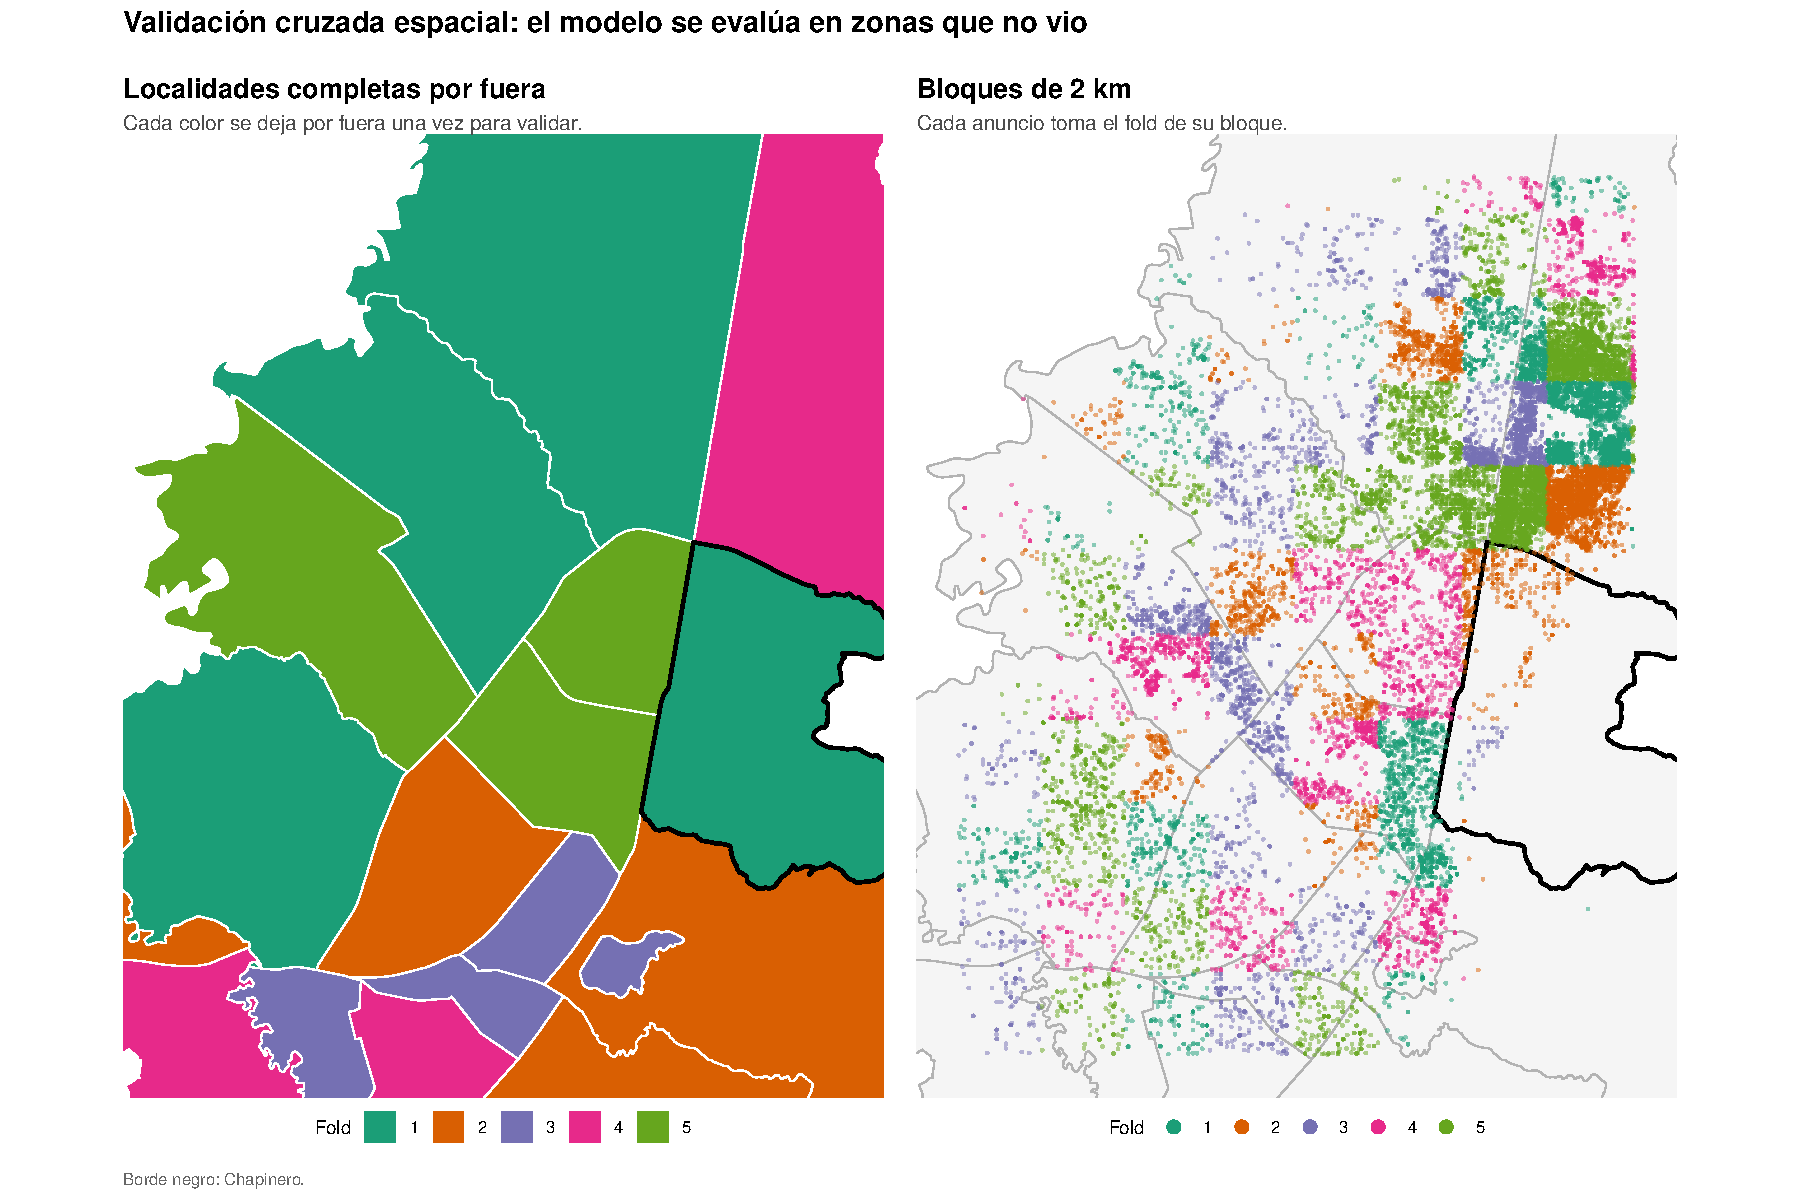
\includegraphics[height=0.86\textheight]{mapa_06_folds_espaciales.pdf}
  \note{En la validación aleatoria, un anuncio de validación casi siempre tiene vecinos en entrenamiento que comparten su precio, y el error se ve más bajo de lo que es. Con localidades completas por fuera, el modelo tiene que predecir una zona que no vio, como pasa con Chapinero. También probamos bloques de 2 km y bloques con un buffer de 300 metros.}
\end{frame}


% --- Comparación de familias --------------------------------------------------
\begin{frame}{Seis familias, un ganador claro: el boosting}
  \centering
  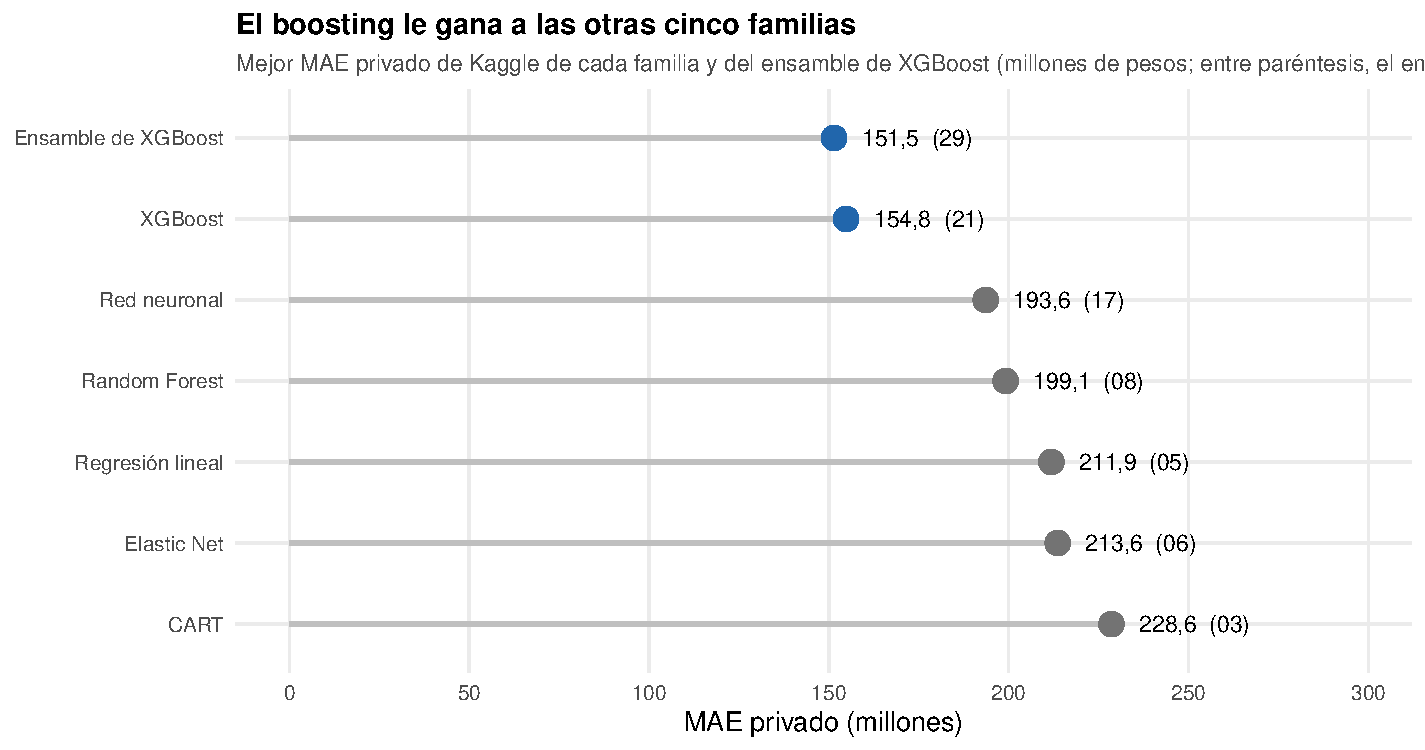
\includegraphics[width=0.85\textwidth]{pres_familias.pdf}
  \lectura{El mejor XGBoost individual ya le gana por más de 35 millones a la mejor alternativa; el ensamble agrega 3 millones más.}
  \note{Se muestra el mejor envío de cada familia en el puntaje privado. Las redes neuronales quedaron cerca del Random Forest, pero muy lejos del boosting. Entre paréntesis está el número del envío.}
\end{frame}

% C6. Escalera del error
\begin{frame}{Cada idea, cuánto bajó el error: los datos importaron más que el algoritmo}
  \centering
  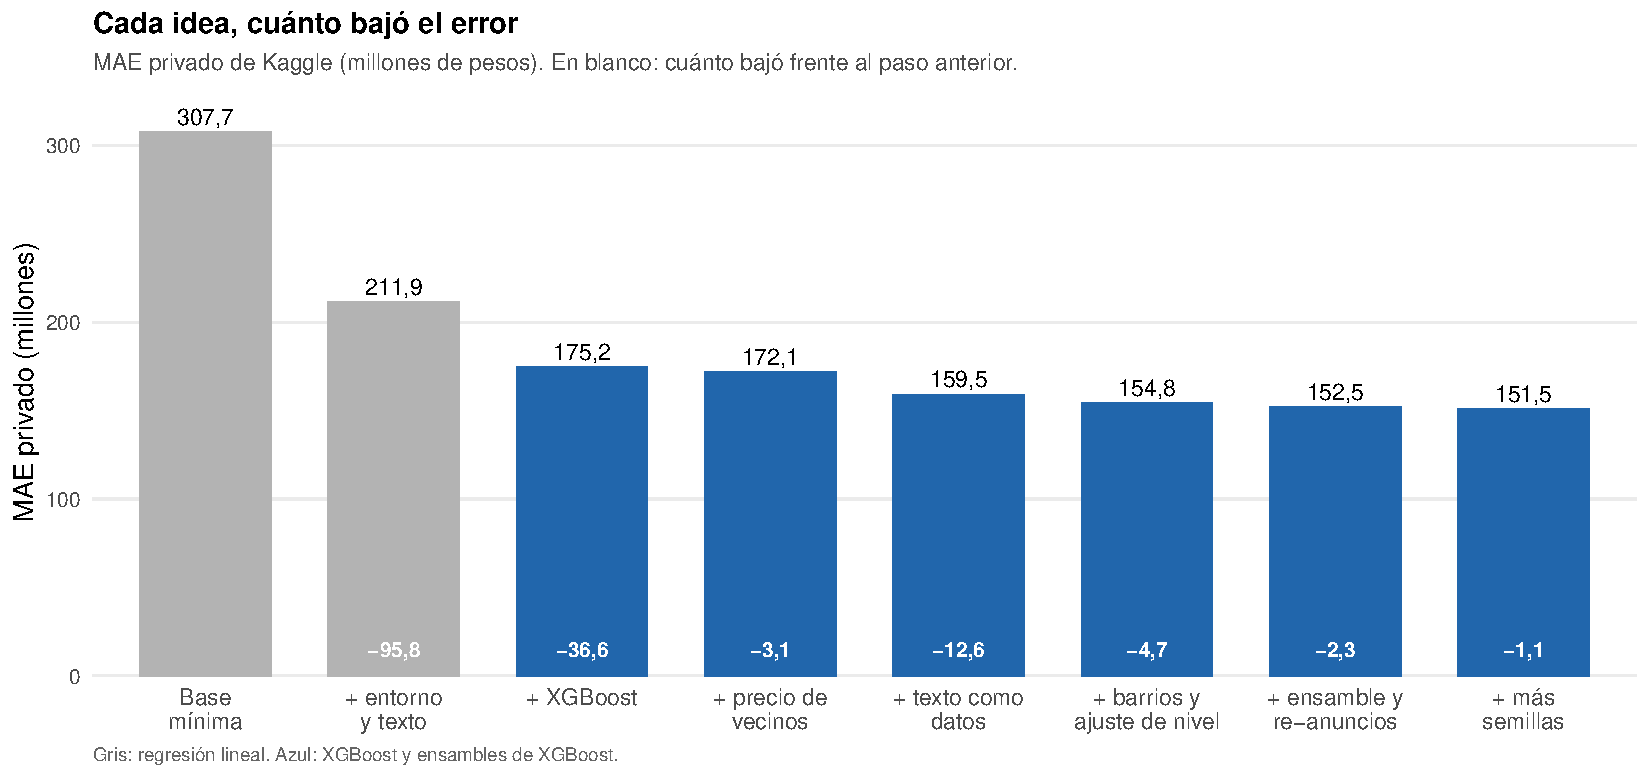
\includegraphics[width=\textwidth]{pres_escalera.pdf}
  \note{Pasar de una base mínima a la base con entorno y texto bajó el error \pasoentorno{} millones. Cambiar la regresión lineal por XGBoost, \pasoxgb{} millones. Después, el texto como datos fue el salto más grande (\pasotexto{} millones). El ensamble, los modelos del precio por m$^2$, las semillas y el ajuste de nivel aportan menos, pero suman. Los embeddings del último paso casi no recibieron peso en el ensamble.}
\end{frame}


\begin{frame}{Por qué pierden los modelos simples}
  \centering
  \figuraancha{pres_modelos_simples.pdf}
  \lectura{La regresión lineal no captura interacciones (el valor de un m$^2$ depende de la zona) y comprime más los extremos; un solo árbol predice pocos precios distintos.}
  \note{Izquierda: error medio por decil de precio con localidades por fuera. Los dos modelos subestiman lo caro, pero la regresión lineal mucho más. Derecha: CART asigna el mismo precio a todos los anuncios de una hoja, así que en test predice solo unos 59 precios distintos. El Elastic Net no ayuda frente a la regresión lineal porque hay muchas más observaciones que variables.}
\end{frame}

\begin{frame}{Con los mismos datos, el algoritmo lo cambia todo}
  \centering
  \resizebox{0.9\textwidth}{!}{\begin{tabular}{lrrrr|r}
\toprule
 & \multicolumn{4}{c|}{Validación cruzada} & Kaggle \\
Familia & Aleatoria & Bloques 2 km & Bloques + buffer & Localidades & privado \\
\midrule
Regresión lineal & 146 & 151 & 153 & 161 & 212 \\
Elastic Net & 146 & 150 & 151 & 158 & 214 \\
CART & 141 & 150 & 153 & 167 & 233 \\
Random Forest & \textbf{103} & 132 & 135 & 146 & 199 \\
XGBoost & 110 & \textbf{125} & \textbf{128} & \textbf{134} & \textbf{175} \\
\bottomrule
\end{tabular}
}

  \vspace{1em}
  \lectura{MAE en millones de pesos. Envíos 05 a 09: misma base y cinco familias. En negrilla, el mejor de cada columna.}
  \note{Esta tabla aísla el efecto del algoritmo: todas las familias usan exactamente las mismas variables. La distancia entre el peor (CART) y el mejor (XGBoost) en Kaggle es de casi 60 millones. Fíjense en la columna aleatoria: ahí el mejor es el Random Forest.}
\end{frame}

\begin{frame}{Qué familia gana según cómo se valida}
  \centering
  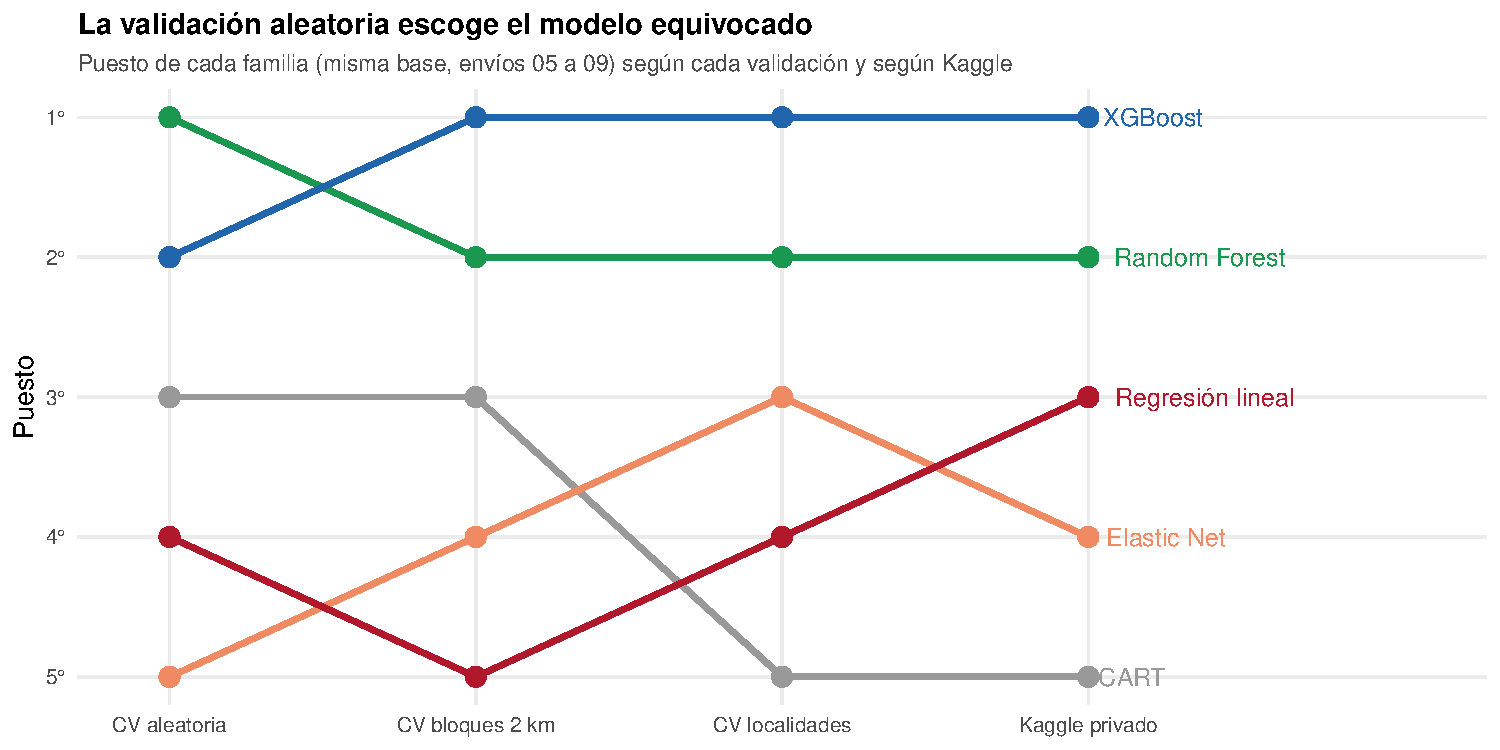
\includegraphics[width=0.88\textwidth]{pres_puestos_validacion.pdf}
  \note{Con la misma base, el Random Forest es el mejor en la validación aleatoria, pero el XGBoost gana en las validaciones espaciales y en Kaggle. El Random Forest memoriza bien a los vecinos, que en la validación aleatoria están en entrenamiento, pero extrapola mal a zonas nuevas. Las dos validaciones no identifican el mismo mejor modelo; la espacial acierta.}
\end{frame}

\begin{frame}
  \centering
  \vspace*{-0.4em}\makebox[\textwidth]{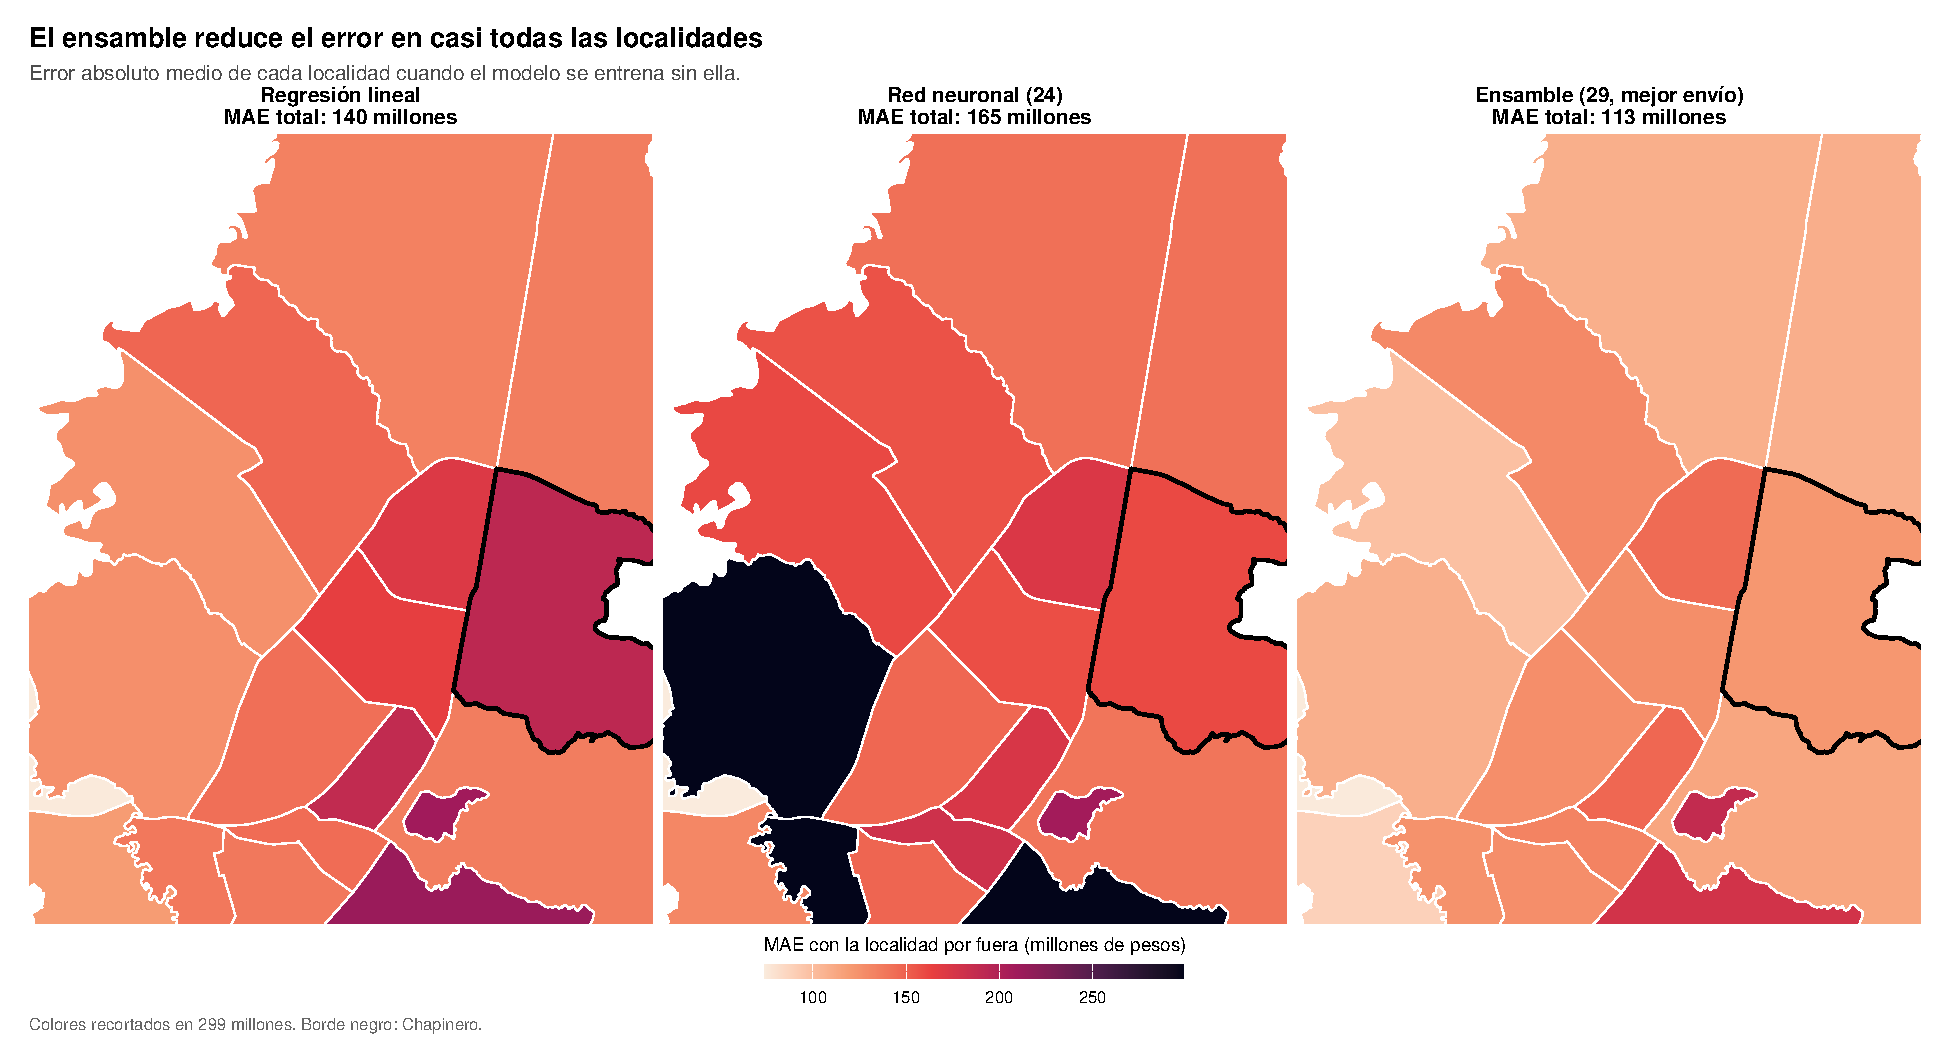
\includegraphics[height=1.01\textheight]{mapa_07_mae_localidad_modelos.pdf}}
  \note{Cada localidad muestra su MAE cuando su grupo de localidades se dejó por fuera del entrenamiento. El ensamble reduce el error en casi todas las localidades, incluidas las del norte, que son las más parecidas a Chapinero.}
\end{frame}

% C8. Pesos por parecido con test
\begin{frame}{Le enseñamos al modelo a mirar lo que se parece a Chapinero}
  \begin{columns}[c]
    \begin{column}{0.5\textwidth}\centering
      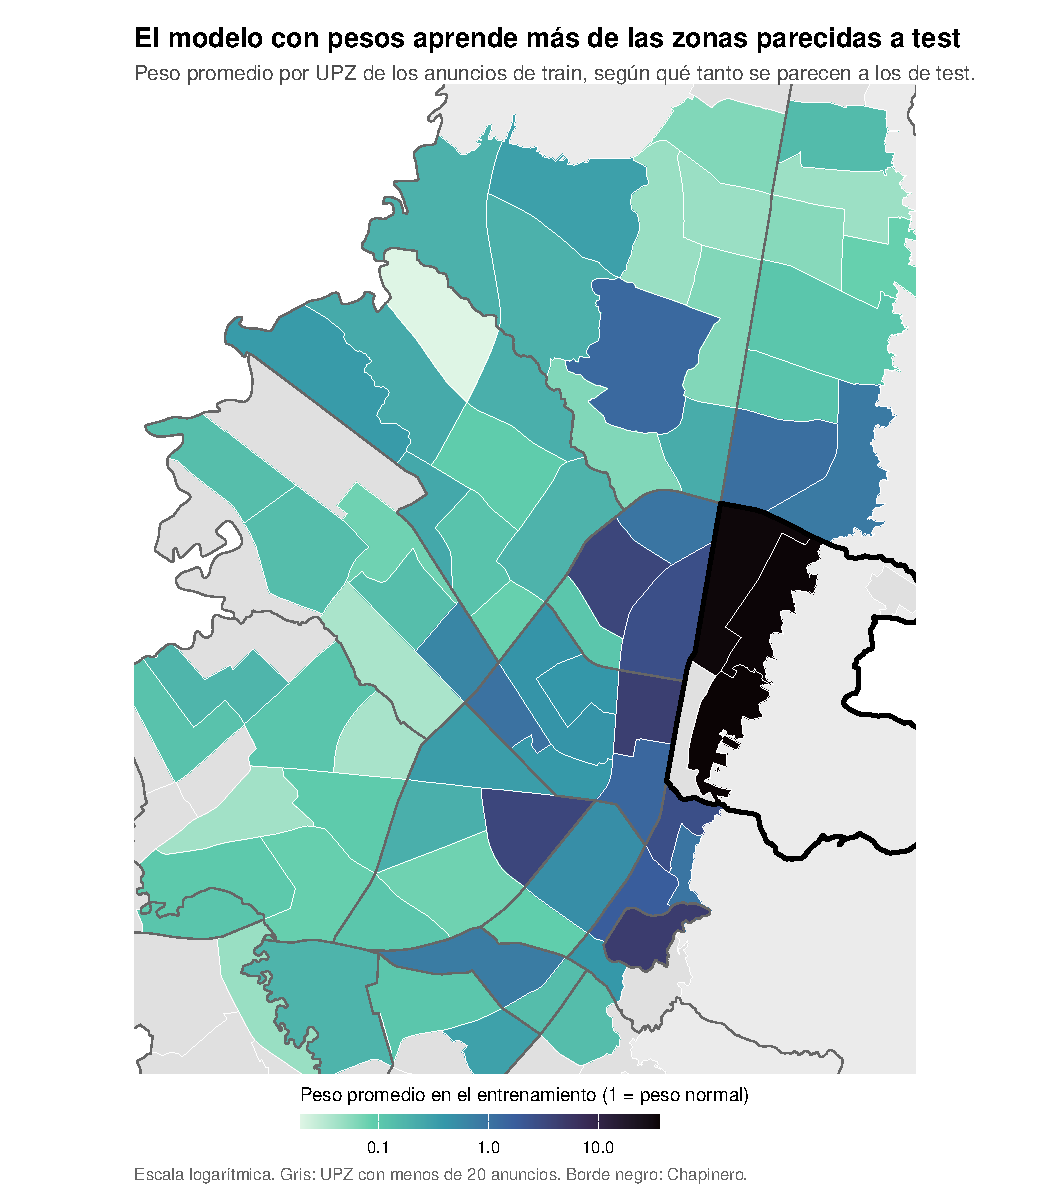
\includegraphics[height=0.82\textheight]{mapa_08_pesos_upz.pdf}
    \end{column}
    \begin{column}{0.45\textwidth}
      \begin{itemize}
        \item Un modelo aprende a distinguir los anuncios de train de los de test.
        \item Los anuncios de train que ``parecen de test'' reciben más peso al entrenar.
        \item Así el modelo dedica más esfuerzo a acertar en viviendas como las de Chapinero.
      \end{itemize}
    \end{column}
  \end{columns}
  \note{Es una forma de corregir el cambio de distribución entre train y test. El peso es la probabilidad de parecerse a test sobre la probabilidad de parecerse a train. En Kaggle los pesos ayudaron unos 3 millones en algunos pares de modelos, pero en el puntaje privado la ganancia no siempre se mantuvo: son diferencias pequeñas.}
\end{frame}


% C5. Qué revela el modelo sobre los precios (interpretación hedónica)
\begin{frame}{Qué revela el modelo: el precio es tamaño, ubicación y lo que dice el anuncio}
  \centering
  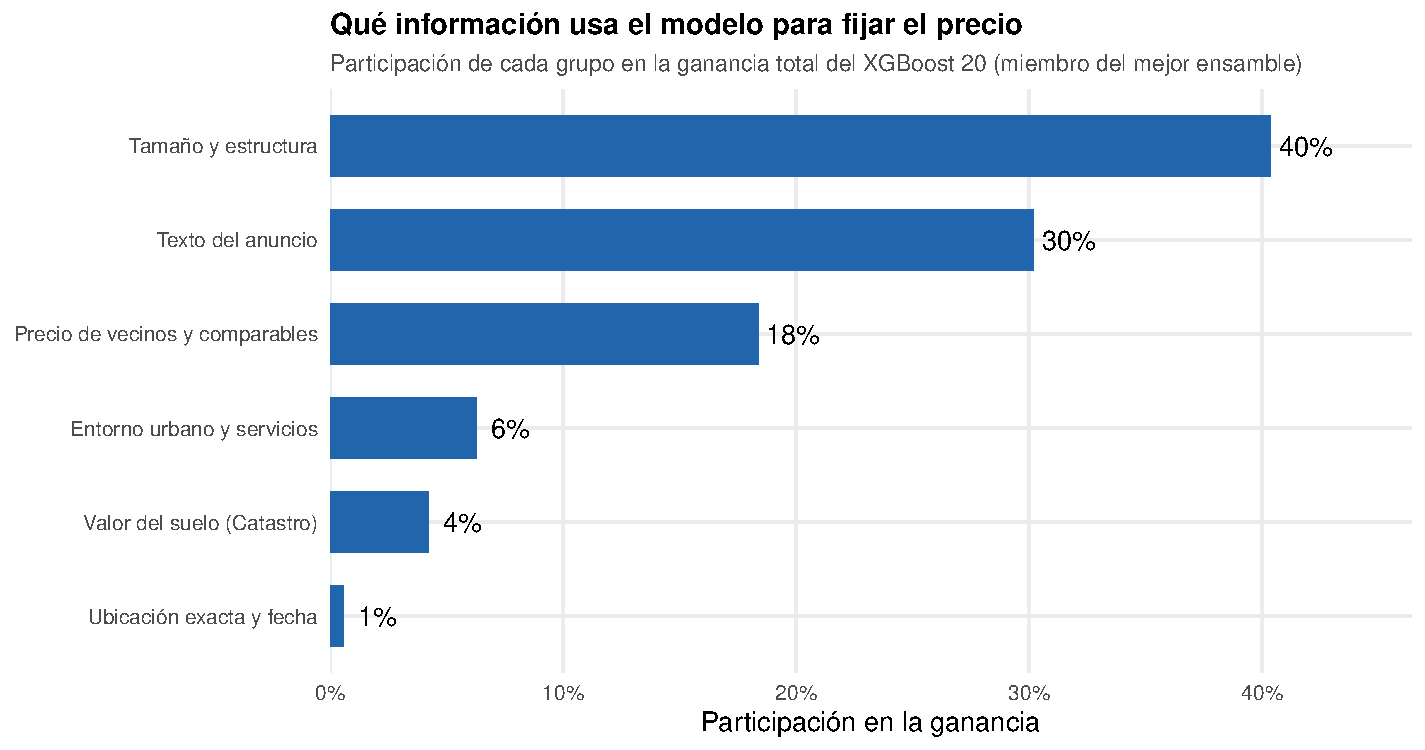
\includegraphics[height=0.8\textheight]{pres_importancia_grupos.pdf}
  \lectura{Como en Rosen (1974), el precio depende de las características de la vivienda y de su entorno. El texto recoge calidad y acabados que ninguna otra variable mide.}
  \note{La ganancia mide cuánto mejora el ajuste cada vez que el modelo usa una variable. El tamaño (área, baños, habitaciones) explica el nivel del precio. El texto es el segundo grupo: dice si el inmueble es de lujo, está remodelado o tiene club house. El precio de los vecinos y el valor del suelo de Catastro resumen la ubicación. Las amenidades sueltas (parques, transporte) pesan poco por separado, porque su efecto ya está en el precio de la zona.}
\end{frame}


% --- Qué significa para el negocio --------------------------------------------
% C9. Kaggle frente a negocio
\begin{frame}{Lo que gana en Kaggle no es lo que gana la empresa}
  \centering
  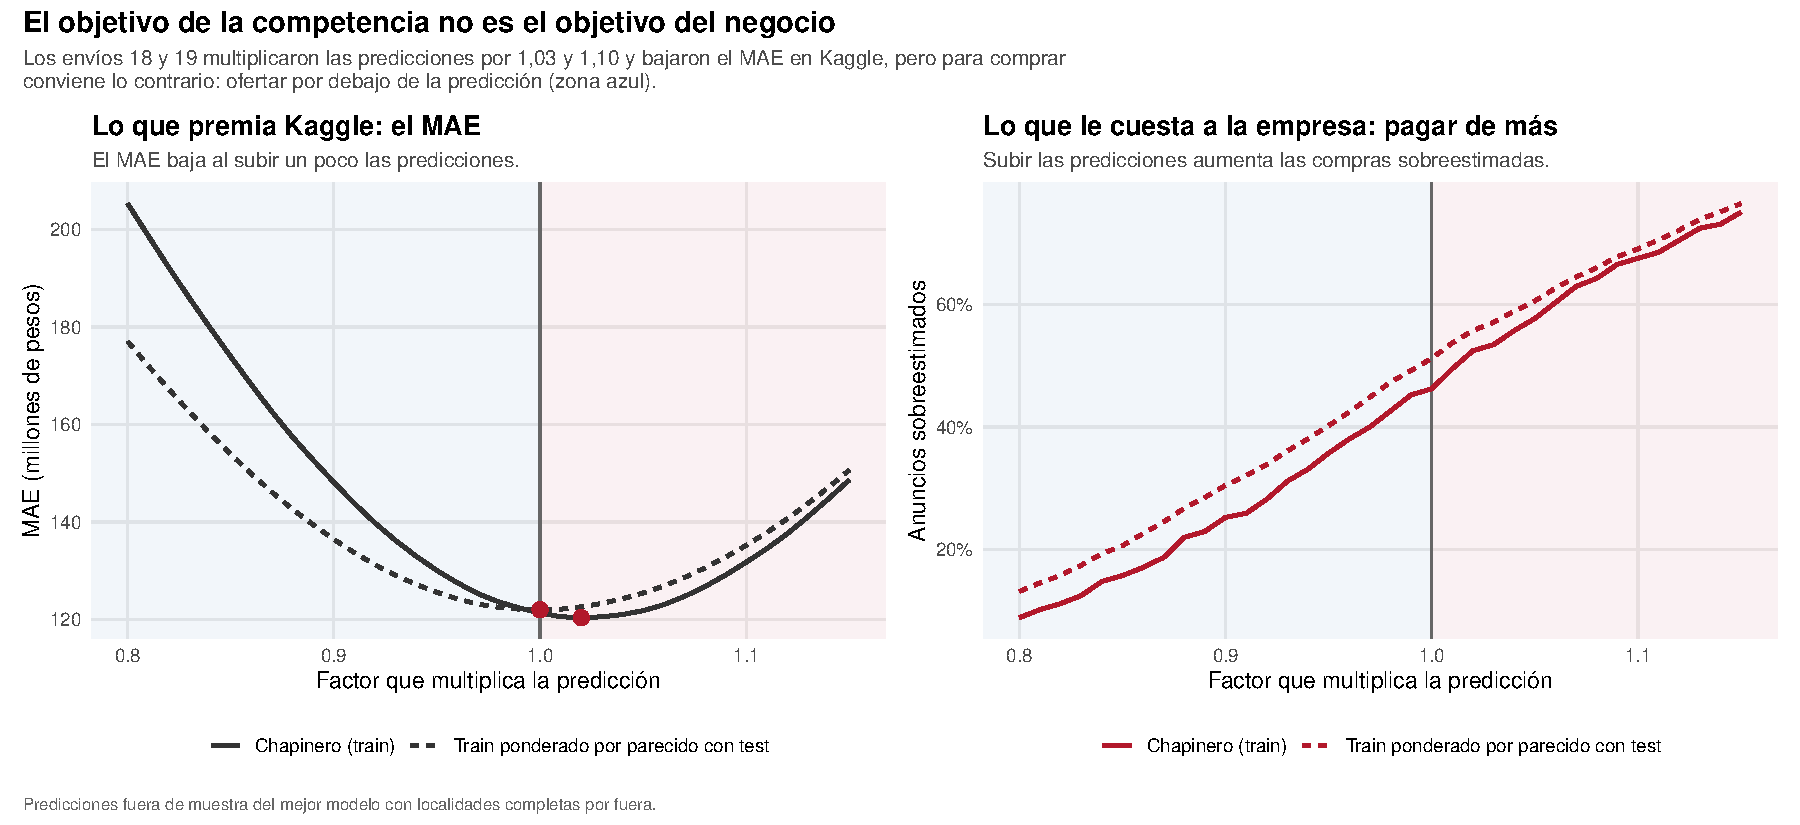
\includegraphics[width=\textwidth]{negocio_05_kaggle_vs_negocio.pdf}
  \note{El modelo subestima Chapinero, así que subir un poco las predicciones bajó el MAE en Kaggle. Pero para la empresa es al revés: sobreestimar significa pagar de más y destruir capital, como le pasó a Zillow; subestimar solo hace perder el negocio. La empresa debe ofertar por debajo de la predicción.}
\end{frame}

% C11. Riesgo de sobreestimación por UPZ
\begin{frame}
  \begin{columns}[c]
    \begin{column}{0.6\textwidth}\centering
      \mapavertical{negocio_01_riesgo_sobreestimacion_upz.pdf}
    \end{column}
    \begin{column}{0.38\textwidth}
      \titulolateral{Dónde pagaríamos de más si compráramos al precio predicho}
      \begin{itemize}\footnotesize
        \item En Chapinero, el \sobrediezchap{} de las viviendas se sobreestima en más de 10\%.
        \item Pagar el precio predicho en esos casos es perder capital.
        \item El riesgo cambia por zona: no sirve un solo margen para toda la ciudad.
      \end{itemize}
    \end{column}
  \end{columns}
  \note{Este es el error que le importa a la empresa: el de sobreestimar. El mapa muestra, por UPZ, el porcentaje de anuncios cuya predicción supera el precio en más de 10\%.}
\end{frame}

% C12. Margen de seguridad por UPZ
\begin{frame}
  \begin{columns}[c]
    \begin{column}{0.6\textwidth}\centering
      \mapavertical{negocio_02_margen_seguridad_upz.pdf}
    \end{column}
    \begin{column}{0.38\textwidth}
      \titulolateral{Margen de seguridad por zona}
      \begin{itemize}\footnotesize
        \item Margen de seguridad: cuánto ofertar por debajo de la predicción para que solo 1 de cada 10 compras pague de más.
        \item En Chapinero: \textbf{\margenchap}.
        \item Donde el modelo se equivoca más, el margen tiene que ser mayor.
      \end{itemize}
    \end{column}
  \end{columns}
  \note{Si q90 es el percentil 90 de la razón entre predicción y precio, el margen es 1 menos 1 sobre q90. Es una regla simple que traduce el error del modelo en una decisión de oferta.}
\end{frame}

% C13. Curva de decisión del margen en Chapinero (selección adversa)
\begin{frame}{La trampa de Zillow: el vendedor acepta cuando el modelo lo favorece}
  \centering
  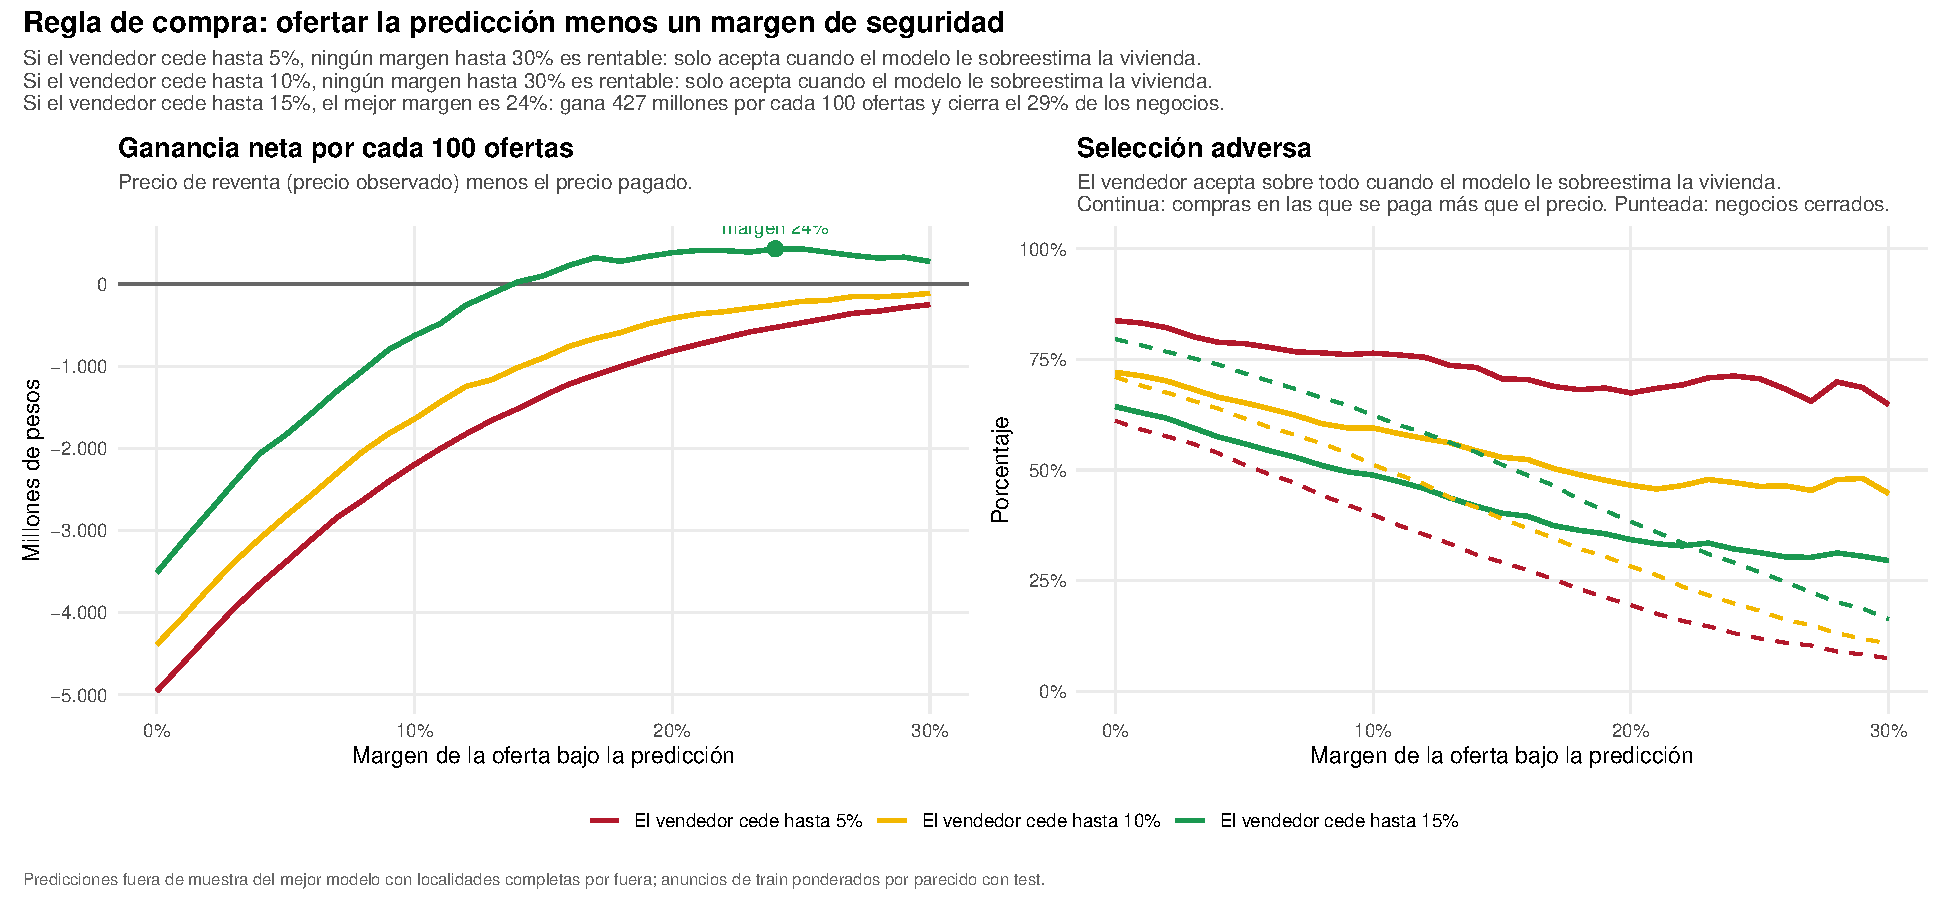
\includegraphics[height=0.8\textheight]{negocio_04_curva_margen.pdf}
  \lectura{En Chapinero, si el vendedor cede hasta \descuentomax, el margen más rentable es \mejormargen{}: \gananciacien{} millones por cada 100 ofertas, cerrando el \negociosmargen{} de los negocios.}
  \note{Selección adversa: los vendedores aceptan nuestra oferta sobre todo cuando el modelo les sobreestima la vivienda, porque en ese caso ofrecemos más de lo que vale. Con descuentos menores, \notadescuentos. Las curvas usan los \nchaptrain{} anuncios de Chapinero en train, por eso no son suaves. Los descuentos que acepta el vendedor son supuestos nuestros, no datos.}
\end{frame}

% C10. Semáforo de compra y recomendación
\begin{frame}{¿Compraríamos? Sí, como filtro y punto de partida, no como precio automático}
  \begin{columns}[c]
    \begin{column}{0.48\textwidth}\centering
      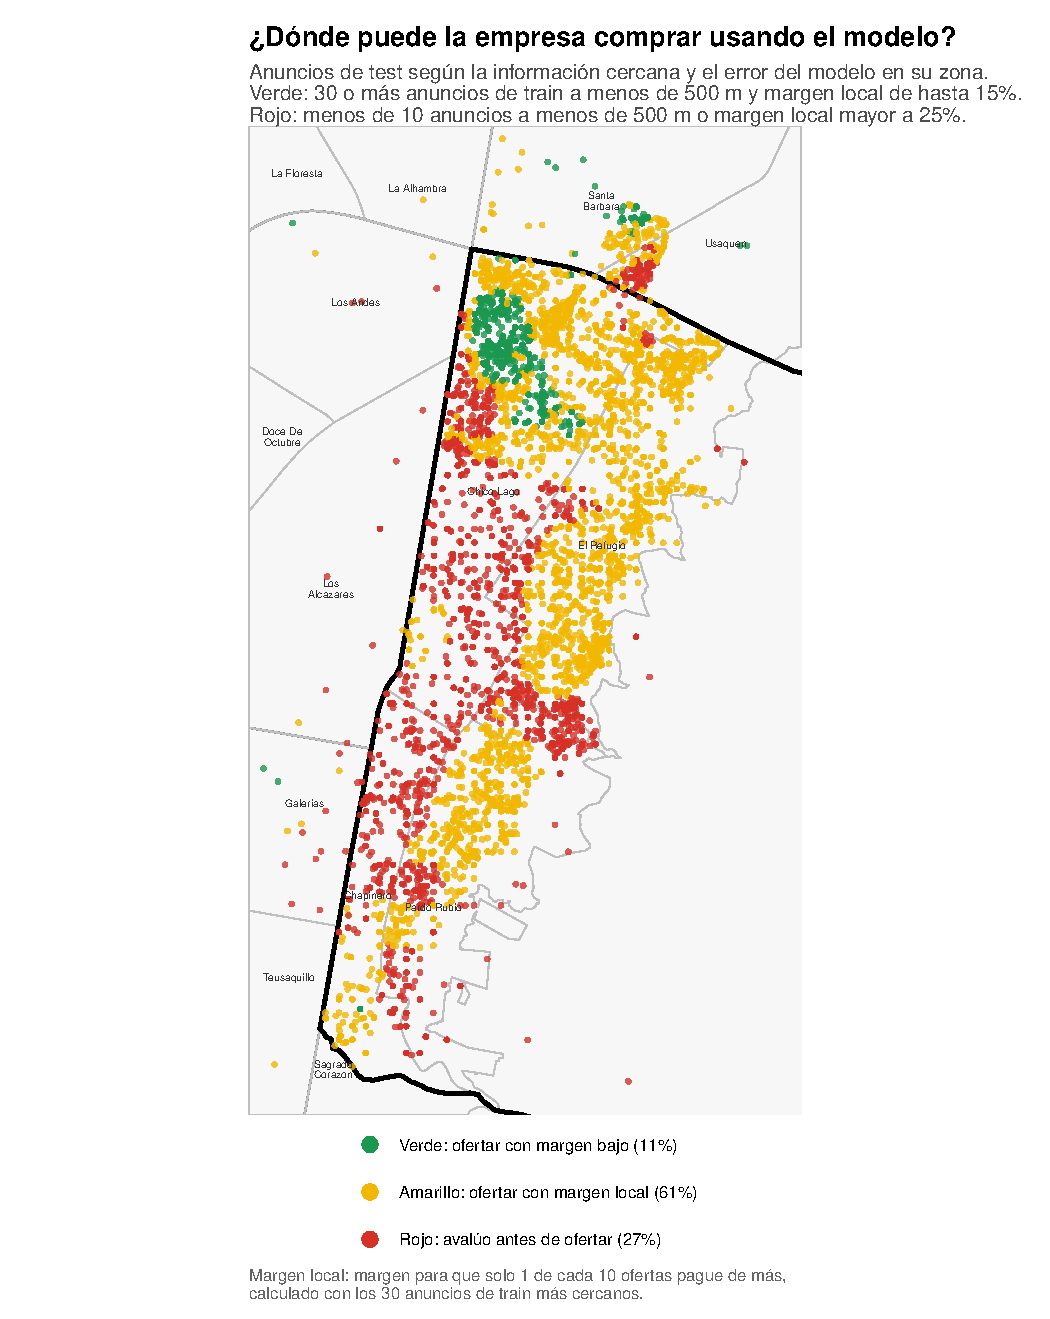
\includegraphics[height=0.84\textheight]{negocio_03_semaforo_test.pdf}
    \end{column}
    \begin{column}{0.5\textwidth}
      \textbf{\color{azul}Recomendación}
      \begin{enumerate}\small
        \item Usar la predicción como valor de referencia y ofertar alrededor de \margenchap{} por debajo.
        \item Verde (\pctverde): ofertar con margen bajo.
        \item Amarillo (\pctamarillo): ofertar con el margen de la zona.
        \item Rojo (\pctrojo): avalúo antes de ofertar.
        \item Monitorear las compras y reentrenar con los precios reales.
      \end{enumerate}
      \vspace{0.3em}
      {\small\color{gris}Riesgo principal: el vendedor acepta justo cuando el modelo le sobreestima la vivienda.}
    \end{column}
  \end{columns}
  \note{El semáforo combina dos cosas: cuántos anuncios de train hay cerca (si hay información) y qué tanto se equivoca el modelo en esa zona. El margen de \margenchap{} hace que solo 1 de cada 10 compras en Chapinero pague más que el precio. La compra automática no es rentable si el vendedor cede poco: los que aceptan son los que el modelo sobrevalora.}
\end{frame}


\end{document}
